\section{Wstęp techonologiczny}\label{sec:geolocalisation_introduction}

Aby poznać lokalizację stacji ISS wykorzystujemy technikę telemetrii opartą o TLE (two-line elements).
Dzięki informacjom zawartym w TLE, można przy użyciu specjalnych programów komputerowych
(np pakiet ephem dostępny w języku programowania Python do wersji 3.4 włącznie)
wyznaczyć dokładne położenie danego satelity w czasie i przestrzeni.

TLE to najbardziej popularny format zapisu elementów orbitalnych sztucznych satelitów Ziemi.
W systemie TLE, w postaci dwóch linii (wierszy) zapisane są parametry keplerowskie orbit
sztucznych satelitów oraz inne informacje takie jak numer satelity w katalogu USSPACECOM
i NORAD, daty wprowadzenia satelity na orbitę i wygenerowania informacji TLE.

\noindent \textit{
\\
ISS \\
1 25544U 98067A 18019.53562654 .00016717 00000-0 10270-3 0 9002 \\
2 25544 51.6396 39.7742 0003526 27.0102 333.1234 15.54187636 15395 \\
}

W systemie tym zawarte są kepleriańskie parametry orbit, czyli orbit stałych (przewidziane
są konkretne zmiany orbity względem czasu). Nieregularności orbitalne sztucznych satelitów,
spowodowane są m.in. wiatrem słonecznym, tarciem atmosferycznym i nieregularnym polem
magnetycznym na różnych szerokościach geograficznych Ziemi. Dlatego elementy orbitalne TLE,
należy często uaktualniać gdyż z biegiem czasu stają się niedokładne i błędnie odzwierciedlają
położenie satelity w przestrzeni. Częściej należy uaktualniać TLE satelitów o niskich orbitach
sięgających do 400 km wysokości (np. ISS) - zaleca się aktualizację co 1-2 tygodnie. TLE satelitów
o wyższych orbitach można uaktualniać odpowiednio, co kilka tygodni, a nawet miesięcy.
System zapisu jest powszechnie używany przez NASA i NORAD, które na bieżąco podają nowe
efemerydy zapisywane w systemie TLE.

Mając dokładną lokalizację stacji ISS w danej chwili możemy oznakować zdjęcie koordynatami
geograficznymi punktu na Ziemi znajdującego się dokładnie pod stacją.

\section{Wyznaczanie horyzontu}\label{sec:geolocalisation_horizon}

Postanowiliśmy dodatkowo wyznaczyć widoczny ze stacji obszar w granicach horyzontu, by lepiej
orientować się w możliwościach kamery znajdującej się na ISS.

Punkt reprezentujemy jako parę współrzędnych wyrażonych w stopniach dziesiętnych (DD - Decimal degrees).
Nie wiedzieć czemu, przyjęło się że we współrzędnych najpierw określamy szerokość (N, S),
a dopiero potem długość (W, E) - odwrotnie niż na układzie współrzędnych.
Ponieważ operujemy w geometrii sferycznej, wzory znane z geometrii euklidesowej nie mają
tutaj zastosowania. W szczególności odległość dwóch punktów o tej samej różnicy drugich współrzędnych,
jest różna i zależy także od pierwszej współrzędnej.

Dzieje się tak, ponieważ reprezentacja w stopniach dziesiętnych zakłada, że mapa jest prostokątna, a
sfery nie da się spłaszczyć bez dodatkowych, zaburzających proporcje mapy operacji. Sferę rozcina
się na płatki (sphere net, gores), i dokonuje ich projekcji i uzupełnienia brakujących fragmentów.

\begin{center}
    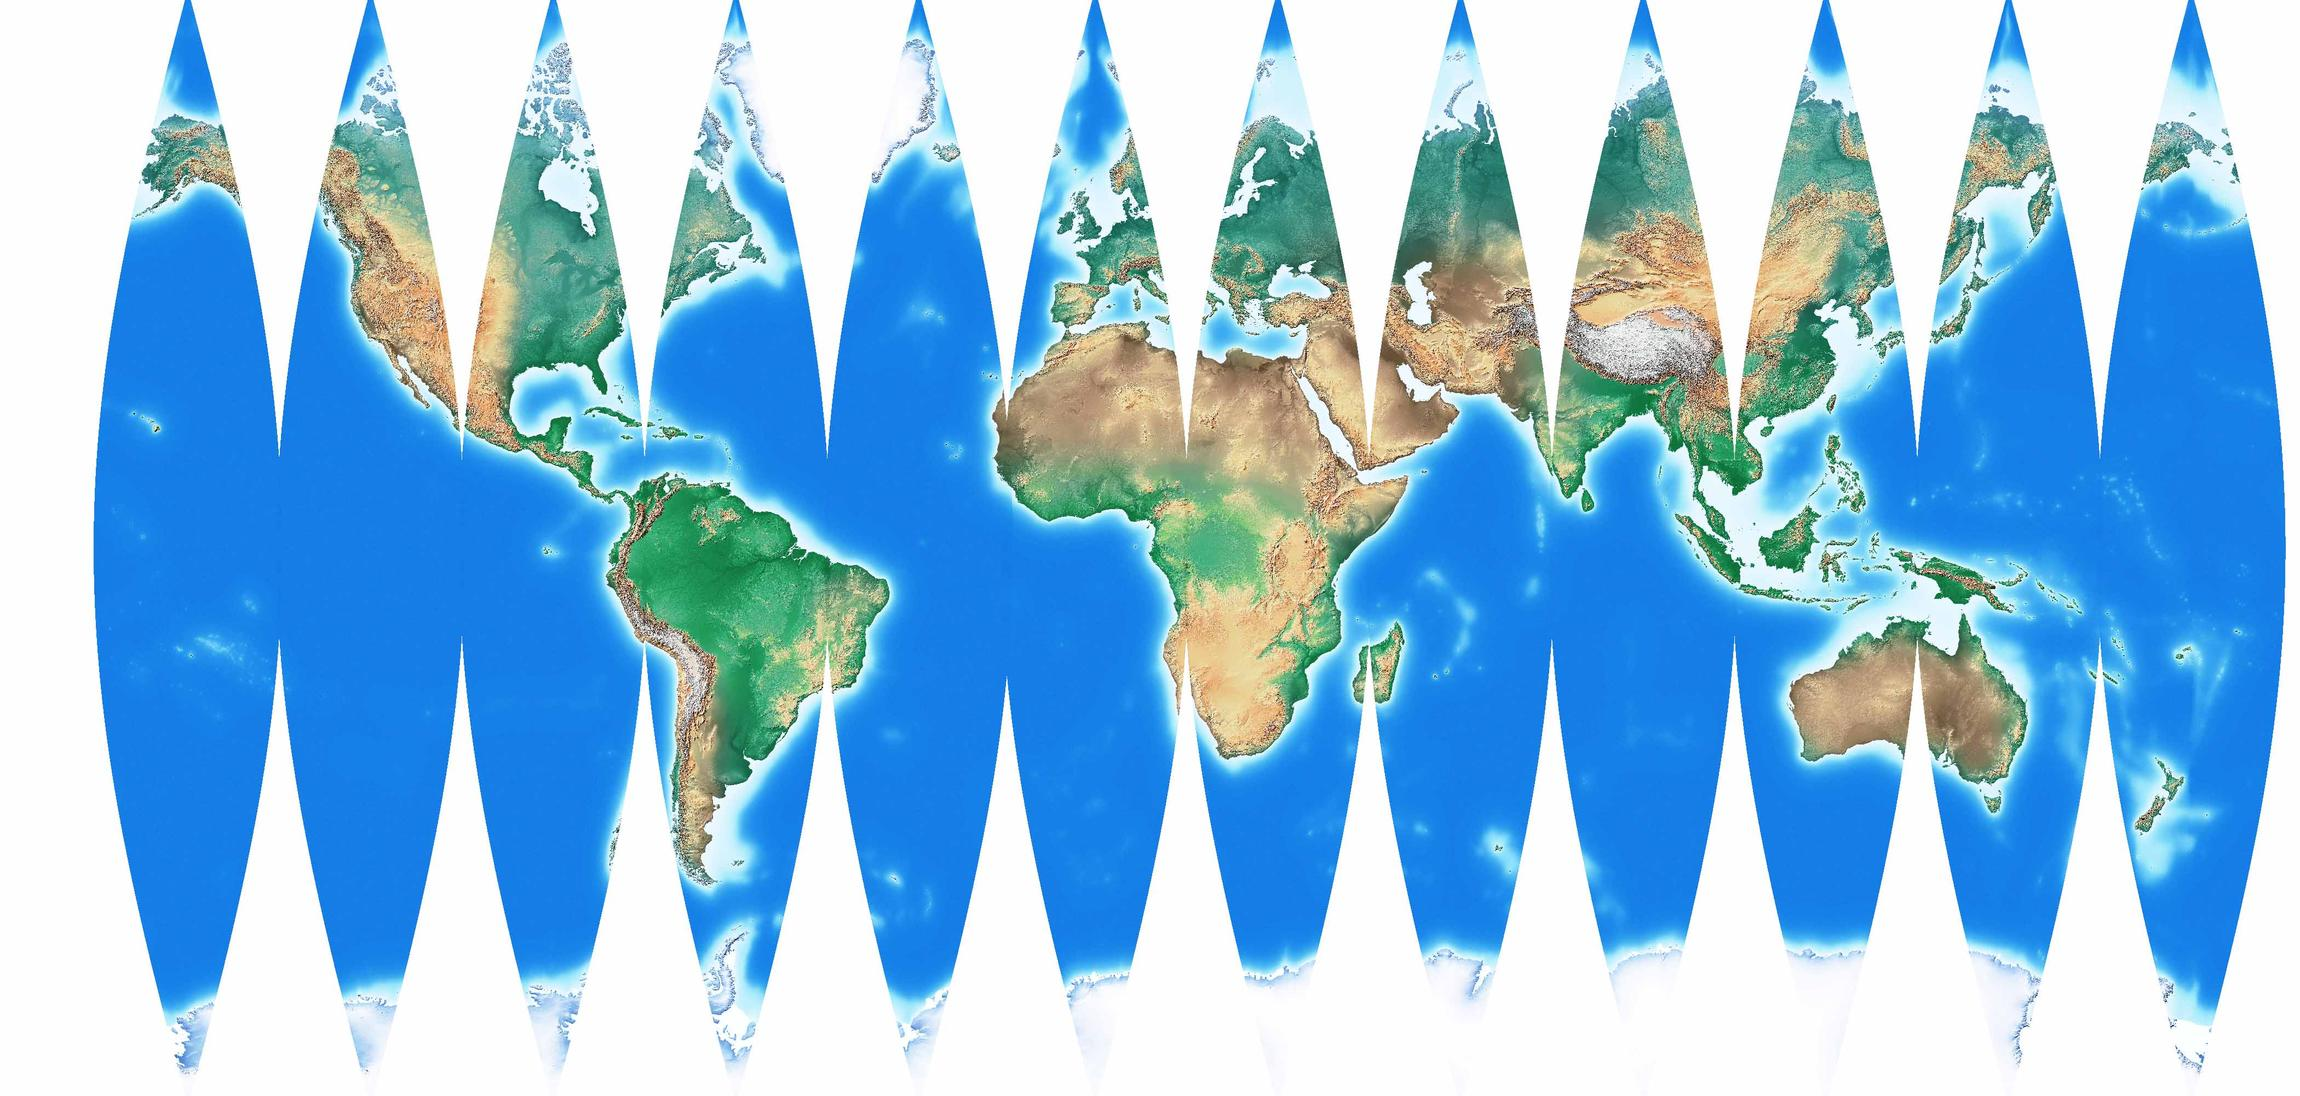
\includegraphics[width=0.9\textwidth]{photos/gores_map.jpg}
    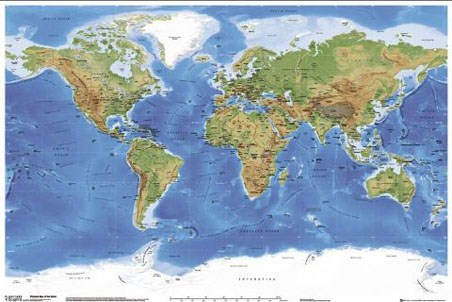
\includegraphics[width=0.9\textwidth]{photos/full_map.jpg}
\end{center}

Naszym celem było wyznaczenie okręgu na sferze, którego środek wypadałby w punkcie bezpośrednio
pod stacją ISS, a obwód wyznaczał horyzont. Okrąg ten chcieliśmy przybliżać wielokątem foremnym.
Ponieważ rozważaliśmy także automatyczne wyznaczanie jakie kraje są widoczne ze stacji w danej
chwili, zdecydowaliśmy się na podział wielokąta na nachodzące na siebie częściowo prostokąty
(by móc sprawdzać czy punkt tworzący granicę kraju jest wewnątrz wielokąta sprawdzalibyśmy czy
zawiera się w którymś z prostokątów).

\begin{figure}[H]
    \begin{subfigure}{0.5\textwidth}
        \centering
        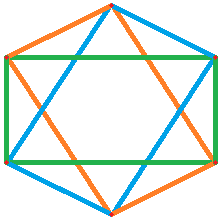
\includegraphics[width=0.9\linewidth]{photos/circle.png}
        \caption{Przykładowy podział wielokąta foremnego na nachodzące prostokąty}
    \end{subfigure}
    \begin{subfigure}{0.5\textwidth}
        \centering
        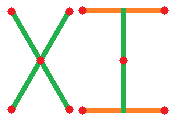
\includegraphics[width=0.9\linewidth]{photos/models.png}
        \caption{Możliwe metody budowania prostokątów}
    \end{subfigure}
\end{figure}

Znaleźliśmy dwa możliwe sposoby modelowania prostokątów, prowadząc z punktu obie przekątne, lub
prowadząc linię równoległą do boków, a później dwie linie prostopadłe do niej. Myśląc także o
innych zastosowaniach naszych algorytmów (np wyznaczania prostokątnego ograniczenia jakiejś
prostej na mapie) zdecydowaliśmy się początkowo na metodę drugą, co ostatecznie okazało się błędem.

\section{W geometrii euklidesowej}\label{sec:geolocalisation_euclidean}

Początkowo, nie zdając sobie sprawy z problemu geometrii sferycznej, zastosowaliśmy twierdzenia
Pitagorasa i wzór na funkcję liniową, by wyznaczyć kolejne prostokąty. Poniższe grafiki przedstawiają
wizualizację punktów w Google Earth. Na pierwszej z nich możemy zaobserwować, że mimo przesunięcia
na górze i na dole o tyle samo punktów dziesiętnych, otrzymaliśmy trapez, a nie prostokąt. Wynika
to z uzupełniania i rozciągania mapy przy spłaszczaniu sfery. W małej skali (gdzie odległości miedzy
punktami wynosiły kilka metrów) otrzymywaliśmy równoległobok, zamiast prostokąta.

Wymyśliliśmy, że możemy przed zastosowaniem operacji znanych z geometrii euklidesowej przeskalować
współrzędne x punktów wejściowych, tak, by kąt prosty był tam, gdzie się go spodziewamy. Po
zastosowniu tych operacji nowe punkty mogliśmy przeskalować odwrotnie. Spodziewaliśmy się
otrzymać prostokąty, nie trapezy. W małej skali (gdy odległości między punktami wynosiły kilka metrów)
wynik był faktycznie znacznie lepszy niż wcześniej. W dużej skali jednak wyniki były jeszcze gorsze, co
widać na drugim obrazku. Punkty były od siebie oddalone o tyle, że każdy z nich musiałby być przeskalowany
przez inną wartość, co psuło ideę naszego pomysłu.

\begin{figure}[H]
    \begin{subfigure}{0.59\textwidth}
        \centering
        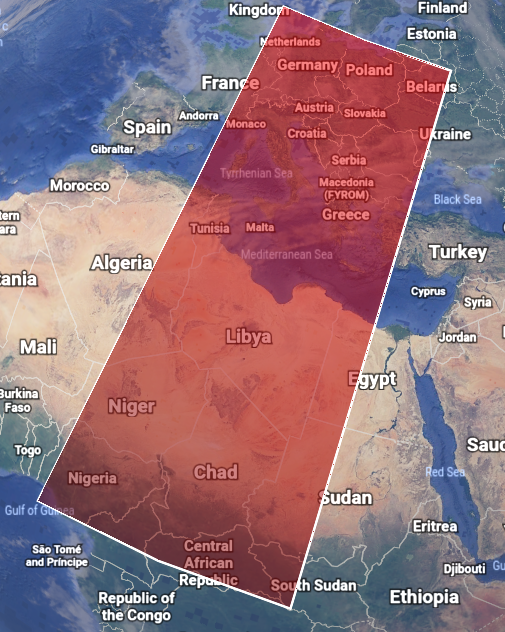
\includegraphics[width=0.9\linewidth]{photos/method1.png}
        \caption{Po zastosowaniu wzorów z geometrii euklidesowej}
    \end{subfigure}
    \begin{subfigure}{0.41\textwidth}
        \centering
        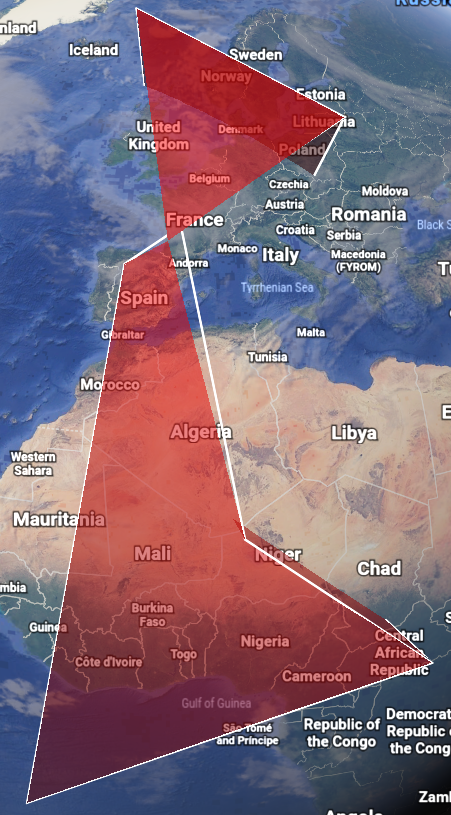
\includegraphics[width=0.9\linewidth]{photos/method2.png}
        \caption{Po wcześniejszym skalowaniu}
    \end{subfigure}
\end{figure}

\section{W geometrii sferycznej}\label{sec:geolocalisation_spherical}

Porzucilismy pomysł korzystania ze znanych nam wzorów i wyszukaliśmy odpowiadające im wzory
w geometrii sferycznej. Pomocna okazała się \href{http://www.movable-type.co.uk/scripts/latlong.html}{ta strona}.

$
\\
\text{W szczególności:} \\
newlat = \arcsin(\sin(lat) \cdot \cos(d) + \cos(lat) \cdot \sin(d) \cdot \cos(bearing)) \\
newlon = lon + \arctan(\sin(bearing) \cdot \sin(d) \cdot \cos(lat), \cos(d) - \sin(lat) \cdot \sin(newlat)) \\
\text{gdzie:} \\
d - \text{odległość do szukanego punktu} \\
lat, lon - \text{współrzędne punktu startowego} \\
bearing - \text{kąt skierowany przeciwnie do wskazówek zegara} \\
\text{między prostą skierowaną na północ i prostą łączącą oba punkty} \\
$

Pozwoliło to znacząco poprawić osiągane wyniki, co można zaobserwować na pierwszej grafice
poniżej. Niestety Wielokąt wciąż nie był idealny. Występowały na nim 'ząbki' wynikające z
różnic rozszerzaniu poszczególnych prostokątów.

Wówczas przypomnieliśmy sobie o drugiej możliwoście generowania prostokątów - bezpośrednio
z przekątnych - co ostatecznie pozwoliło uzyskać porządany od początku wynik.

\begin{figure}[H]
    \begin{subfigure}{0.5\textwidth}
        \centering
        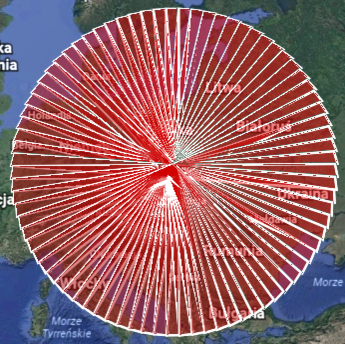
\includegraphics[width=0.9\linewidth]{photos/method3.png}
        \caption{Po zastosowaniu wzorów sferycznych}
    \end{subfigure}
    \begin{subfigure}{0.5\textwidth}
        \centering
        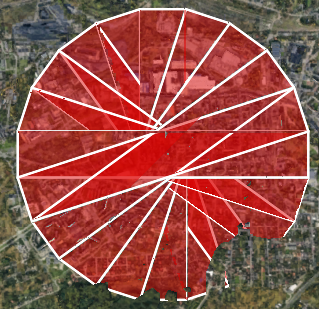
\includegraphics[width=0.9\linewidth]{photos/method4.png}
        \caption{Po zmianie metody budowania prostokątów}
    \end{subfigure}
\end{figure}

ESA poinformowało nas później, że nie jesteśmy w stanie fotografować ze stacji całego widocznego
horyzontu, a jedynie obszar bezpośrednio widziany z okna w którym umiejsciowiony jest mikrokomputer
Raspberry, więc ostatecznie nie wykorzystaliśmy tych obliczeń. Uważamy jednak że poświęcony czas
nie poszedł na marne, nauczyliśmy się bardzo dużo o geometriach nieeuklidesowych.
